% !TEX root = ../main.tex
\documentclass[../main.tex]{subfiles}

\begin{document}

Die Nachfolgende Tabelle zeigt die Anforderungsliste des Pfadfinder-Fahrzeugs.

\textbf{Version 0}

\textbf{Legende} \\ F = Festanforderung \\ M = Mindestanforderung \\ W = Wunschanforderung

\subsection{Allgemeine Anforderungen}
\begin{tabular}{|l|l|l|l|}
  \hline
  & \textbf{F} & & \textbf{Daten} \\
  \textbf{Nr.} & \textbf{M} & \textbf{Bezeichnung} & \textbf{Werte} \\
  & \textbf{W} & & \textbf{Erläuterungen} \\
  \hline
  1.1 & W & Wettbewerb & Team 10 wird im Wettbewerb einen Podestplatz
  erreichen. \\
  \hline
  1.2 & F & Wettbewerbsort & Vorraussichtlich wird der Wettbewerb im
  Foyer der \\
  & & & Mensa durchgeführt. \\
  \hline
  1.3 & F & Projektabgabe & Der PREN 1 Schlussbericht ist bis zum 10.
  Januar 2025 \\
  & & PREN 1 & abzugeben. \\
  \hline
  1.4 & F & Eigenkonstruktion & Einzelne Systemkomponenten wie z.B.
  Räder, Servos, \\
  & & & Motoren, Mikrocontroller, Kamera, etc. dürfen zugekauft \\
  & & & und eingesetzt werden. Das zu realisierende Fahrzeug \\
  & & & als Grosses und Ganzes muss jedoch zwingend eine \\
  & & & Eigenkonstruktion sein. \\
  \hline
  1.5 & F & Software & Es dürfen Software-Komponenten und Software-Services \\
  & & & von Fremd-Herstellern verwendet werden. \\
  \hline
  1.6 & F & Eingriffe & Ein Eingreifen auf das Fahrzeug ist nach dem
  Start nicht \\
  & & & mehr erlaubt. \\
  \hline
  1.7 & F & Sicherheit & Das Team ist während sämtlichen Betriebs- und \\
  & & & Test-Phasen verantwortlich für die Sicherheit des \\
  & & & Fahrzeuges und den Schutz der Personen. \\
  \hline
  1.8 & W & Nachhaltigkeit & Bei Projektentscheiden soll die Nachhaltigkeit \\
  & & & berücksichtigt und auch entsprechend dokumentiert \\
  & & & werden. \\
  \hline
\end{tabular}

\subsection{Gerät}
\begin{tabular}{|l|l|l|l|}
  \hline
  & \textbf{F} & & \textbf{Daten} \\
  \textbf{Nr.} & \textbf{M} & \textbf{Bezeichnung} & \textbf{Werte} \\
  & \textbf{W} & & \textbf{Erläuterungen} \\
  \hline
  2.1 & F & Autonomität & Das Fahrzeug muss den vorgegebenen Parcours
  von Start \\
  & & & bis Ziel ohne Zugriff von aussen absolvieren können. \\
  \hline
  2.2 & F & Hardware- & Alle zum Betrieb benötigten Hardware-Komponenten wie \\
  & & Komponenten & z.B. Sensoren, Aktoren, Steuergeräte, Kamera, etc. \\
  & & & müssen sich im oder auf dem Fahrzeug befinden. \\
  \hline
  2.3 & M & Betriebsbereitschaft & Das Fahrzeug muss innerhalb von
  maximal einer Minute \\
  & & & im Startbereich platziert, aufgebaut und betriebsbereit \\
  & & & sein konnen. \\
  \hline
  2.4 & F &  Gesperrte Wegpunkte & Die gesperrten Wegpunkte müssen
  vom Fahrzeug erkannt \\
  & & & werden. \\
  \hline
  2.5 & F & Hindernis auf & Mögliche Hindernisse müssen vom Fahrzeug erkannt \\
  & & Strecke & werden. \\
  \hline
  2.6 & F & Hindernisbewältigung & Befährt das Fahrzeug eine Strecke
  mit einem Hindernis, \\
  & & & so muss dieses erkannt und aktiv von der Strecke \\
  & & & aufgenommen werden. Sobald das Fahrzeug die besagte \\
  & & & Stelle passiert hat, muss das Hindernis wieder an die \\
  & & & Ursprungsposition zurückgestellt werden. Die \\
  & & & Toleranzzone beim zurückstellen des Hindernis beträgt \\
  & & & 20 mm (umlaufend). \\
  \hline
  2.7 & F & Zielposition & Die Zielposition (1, 2 oder 3) muss am
  Fahrzeug mittels \\
  & & & einem Wahlschalter ausgewählt werden können. \\
  \hline
  2.8 & F & Startbefehl & Der Startbefehl wird mittels einem Schalter
  oder Taster \\
  & & & am Fahrzeug erteilt. (Gleichzeitig wird die Sicht auf \\
  & & & die Strecke freigegeben und die Zeitmessung gestartet) \\
  \hline
  2.9 & F & Leitlinien & Das Fahrzeug muss sich während dem gesamten Parcours \\
  & & & auf den vorgegebenen Leitlinien bewegen. \\
  \hline
  2.10 & F & Not-Aus & Das Fahrzeug muss über einen leicht zugänglichen \\
  & & & Not-Aus-Knopf oder -Schalter verfügen, der alle \\
  & & & mechanisch-dynamische Prozesse sofort unterbricht. \\
  \hline
  2.11 & M & Gewicht & Das Fahrzeug darf das Maximalgewicht von 2kg nicht \\
  & & & überschreiten. \\
  \hline
\end{tabular}

\newpage

\begin{tabular}{|l|l|l|l|}
  \hline
  & \textbf{F} & & \textbf{Daten} \\
  \textbf{Nr.} & \textbf{M} & \textbf{Bezeichnung} & \textbf{Werte} \\
  & \textbf{W} & & \textbf{Erläuterungen} \\
  \hline
  2.12 & M & Dimensionen & Das Fahrzeug darf die Dimensionen des
  Startbereichs \\
  & & & (30 x 30 cm) nicht überschreiten. Zudem ist die Höhe \\
  & & & des Fahrzeugs (oder allfälliger Anbauteile) auf maximal \\
  & & & 80 cm beschränkt. \\
  \hline
  2.13 & F & Zielposition & Das Erreichen der Zielposition muss vom
  Fahrzeug in \\
  & & & einer passenden Form visuell oder akustisch angezeigt \\
  & & & werden. Zudem muss das Fahrzeug innerhalb eines \\
  & & & Kreises von 30 cm Durchmesser um den Zielpunkt zum \\
  & & & Stehen kommen. \\
  \hline
  2.14 & W & Energieversorgung & Die Energieversorgung soll mit einem
  Akku realisiert \\
  & & & werden, der über eine USB-Schnittstelle wieder \\
  & & & aufgeladen werden kann. \\
  \hline
  2.15 & W & Akkulaufzeit & Im aktiven Betrieb des Fahrzeugs soll
  eine Akkulaufzeit \\
  & & & von mindestens 25 Minuten gewährleistet sein. \\
  \hline
  2.16 & W & Debug-Schnittstelle & Die Elektronik des Fahrzeugs soll
  über eine Debug- \\
  & & & Schnittstelle verfügen, die es ermöglicht aktuelle \\
  & & & Zustände und Signale auszulesen. \\
  \hline
\end{tabular}

\subsection{Parcours}
\begin{tabular}{|l|l|l|l|}
  \hline
  & \textbf{F} & & \textbf{Daten} \\
  \textbf{Nr.} & \textbf{M} & \textbf{Bezeichnung} & \textbf{Werte} \\
  & \textbf{W} & & \textbf{Erläuterungen} \\
  \hline
  3.1 & F & Wege-Netzwerk & Das Wege-Netzwerk und der Startpunkt sind
  bekannt. \\
  & & & (Figure \ref{fig:wege-netzwerk}) \\
  \hline
  3.2 & F & Zielpunkte & Die möglichen Zielpunkte sind bekannt, doch der \\
  & & & definitive Zielpunkt wird erst unmittelbar vor dem Start \\
  & & & des Parcours bekannt gegeben. (Figure \ref{fig:wege-netzwerk}) \\
  \hline
  3.3 & F & Wegpunkte & Insgesamt gibt es acht Wegpunkte. Die Wegpunkte sind \\
  & & & aufgeklebte Vollkreise (weiss) mit einem Durchmesser \\
  & & & von 7 bis 12 cm. (Figure \ref{fig:wegpunkt}) \\
  \hline
  3.4 & F & Untergrund & Der Untergrund entspricht dem Bodenbelag des Foyers \\
  & & & der Mensa auf dem Campus der Hochschule Luzern für \\
  & & & Technik und Architektur in Horw. (Figure \ref{fig:fliesenboden}) \\
  \hline
  3.5 & F & Leitlinien & Die Wegpunkte sind mit hellen Leitlinien
  (aufgeklebtes \\
  & & & Klebeband) verbunden. Die Breite der Leitlinien beträgt \\
  & & & ca. 20 mm. \\
  \hline
  3.6 & F & Abmessungen & Der Abstand der Wegpunkte ist variabel zwischen \\
  & & & 0.5 bis 2.0 m. Die Gesamtfläche des Wege-Netzwerkes \\
  & & & beträgt ca. 4.5 x 4.5 m. \\
  \hline
  3.7 & F &  Gesperrte Wegpunkte & Die gesperrten Wegpunkte dürfen
  nicht befahren werden. \\
  & & & Sie sind bis zum Start unbekannt und mittels einem \\
  & & & Leitkegel gekennzeichnet. \\
  \hline
  3.8 & F & Hindernis auf & Die Strecke darf befahren werden, doch
  das Hindernis \\
  & & Strecke & muss aktiv von der Strecke aufgenommen und am \\
  & & & gleichen Ort wieder zurückgestellt werden. \\
  \hline
  3.9 & F & Nicht vorhandene & Leitlinien können aus dem
  Wege-Netzwerk entfernt \\
  & & Teilstrecken & werden. Die entsprechenden Verbindungen können nicht \\
  & & & befahren werden. \\
  \hline
  3.10 & F & Streckenbedingungen & Die Streckenbedingungen (Sperrung,
    Hindernisse, nicht \\
  & & & vorhandene Teilstrecke) sind bis zum Start unbekannt. \\
  \hline
  3.11 & F & Startbereich & Die Grösse des Startbereichs beträgt 30 x
  30 cm. Das \\
  & & & Fahrzeug darf diese Dimensionen nicht überschreiten. \\
  \hline
  3.12 & F & Start & Sobald die Sicht auf die Strecke freigegeben
  wird, beginnt \\
  & & & ebenfalls die Zeitmessung. \\
  \hline
  3.13 & M & Parcours-Laufzeit & Die Laufzeit von Start bis Ziel darf
  maximal vier \\
  & & & Minuten betragen. Wird das Ziel innert vier Minuten \\
  & & & nicht erreicht, ist der Lauf ungültig. \\
  \hline
\end{tabular}

\subsection{Simulation}
\begin{tabular}{|l|l|l|l|}
  \hline
  & \textbf{F} & & \textbf{Daten} \\
  \textbf{Nr.} & \textbf{M} & \textbf{Bezeichnung} & \textbf{Werte} \\
  & \textbf{W} & & \textbf{Erläuterungen} \\
  \hline
  4.1 & W & Betriebssystem & Die Simulation soll auf Linux und auch Windows \\
  & & & ausführbar sein. \\
  \hline
  4.2 & W & Benutzeroberfläche & Die Benutzeroberfläche soll beliebig
  editierbar sein. Die \\
  & & & Die gesamte Simulation wird jedoch nur 2-dimensional \\
  & & & realisiert. \\
  \hline
  4.3 & W & Pfadfindungs- & In der Simulation sollen verschiedene
  Pfadfindungs- \\
  & & algorithmen & algorithmen (z.B. Dijkstra, A*-Algorithmus, etc.) \\
  & & & implementiert werden für eine direkte Gegenüberstellung. \\
  \hline
  4.4 & W & Zeitauswertung & In der Simulation soll eine approximierte \\
  & & & Zeitauswertung, basierend auf heuristischen Abschätzungen, \\
  & & & möglich sein. \\
  \hline
  4.5 & W & Echtzeit- & Der simulierte Pfad soll in Echtzeit
  visualisiert werden, \\
  & & Visualisierung & um das Verhalten des Fahrzeugs besser nachvollziehen \\
  & & des Pfades & zu können. \\
  \hline
  4.6 & W & Hindernistypen & Verschiedene Arten von Hindernissen
  (beweglich und \\
  & & & stationär) sollen simuliert werden können. \\
  \hline
  4.7 & W & Fahrzeugparameter & Fahrzeugparameter (Geschwindigkeit,
    Wendekreis, \\
  & & & Sensorreichweite, etc.) sollen editierbar sein. \\
  \hline
  4.8 & W & Datenexport & Die Daten, welche während der Simulation generiert \\
  & & & werden, sollen exportierbar sein. (z.B. Log-File) \\
  \hline
  4.9 & W & Error-Handling & Der Simulator muss robust auf Fehler
  reagieren und \\
  & & & darf keinesfalls abstürzen. Zudem sollen Fehlerzustände \\
  & & & abgefangen und klar dokumentiert werden. \\
  \hline
\end{tabular}

\subsection{Herstellungsressourcen}
\begin{tabular}{|l|l|l|l|}
  \hline
  & \textbf{F} & & \textbf{Daten} \\
  \textbf{Nr.} & \textbf{M} & \textbf{Bezeichnung} & \textbf{Werte} \\
  & \textbf{W} & & \textbf{Erläuterungen} \\
  \hline
  5.1 & W & Materialbeschaffung & Materialien und Komponenten sollen
  vorzugsweise von \\
  & & & folgenden Lieferanten bestellt werden: \\
  & & & - Conrad Electronic \\
  & & & - Distrelec \\
  & & & - Mädler \\
  & & & - Farnell \\
  \hline
  5.2 & F & Budget & Für die Realisierung des Projekts stehen dem Team \\
  & & & insgesamt 500 CHF zur Verfügung. Davon dürfen maximal \\
  & & & 200 CHF in PREN 1 ausgegeben werden. \\
  \hline
  5.3 & F & Normteile ab HSLU & Normteile (Schrauben, Lager,
    Rohmaterial, Widerstände, \\
  & & Lagerbestand & Kondensatoren, etc.) aus dem HSLU Lagerbestand \\
  & & & dürfen kostenlos verwendet werden. \\
  \hline
  5.4 & F & Persönlicher & Wird für das Projekt ein persönlicher 3D-Drucker \\
  & & 3D-Drucker & verwendet, so muss die verarbeitete Menge \\
  & & & ausgewiesen werden. \\
  \hline
  5.5 & F & Herstellungs- & Dem Team stehen für die Umsetzung des Projekts \\
  & & ressourcen der & (PREN 1 und PREN 2) die folgenden Ressourcen der \\
  & & HSLU & HSLU zur Verfügung: \\
  & & & - maximal 25 h Maschinenlaufzeit der 3D-Drucker \\
  & & & - maximal 1 h Maschinenlaufzeit des Lasergeräts \\
  & & & - maximal 10 Arbeitsstunden des Werkstattpersonals \\
  & & &   Elektrotechnik \\
  & & & - maximal 10 Arbeitsstunden des Werkstattpersonals \\
  & & &   Maschinentechnik \\
  \hline
\end{tabular}

\newpage

\subsection{Abbildungen}
Folgend sind sämtliche Abbildungen aufgeführt, auf die in der
Anforderungsliste referenziert wurde.

\begin{figure} [ht]
  \centering
  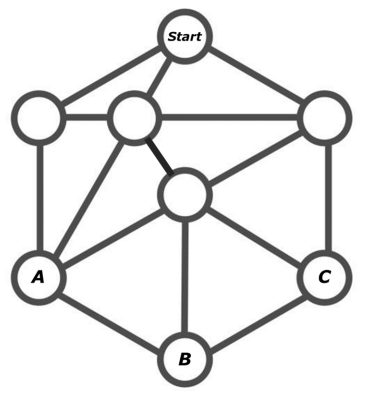
\includegraphics[scale=0.5]{../resources/WegeNetzwerk.png}
  \caption{Vorgegebenes Wege-Netzwerk mit Start- und Zielpositionen A-B-C}
  \label{fig:wege-netzwerk}
\end{figure}

\begin{figure} [ht]
  \centering
  
\includegraphics[scale=0.5]{../resources/Wegpunkt.png}
  \caption{Typischer aufgeklebter Wegpunkt}
  \label{fig:wegpunkt}
\end{figure}

\begin{figure} [ht]
  \centering
  
\includegraphics[scale=0.05]{../resources/Fliesenboden.jpg}
  \caption{Fliesenboden im Foyer der Mensa}
  \label{fig:fliesenboden}
\end{figure}

\newpage

\end{document}
